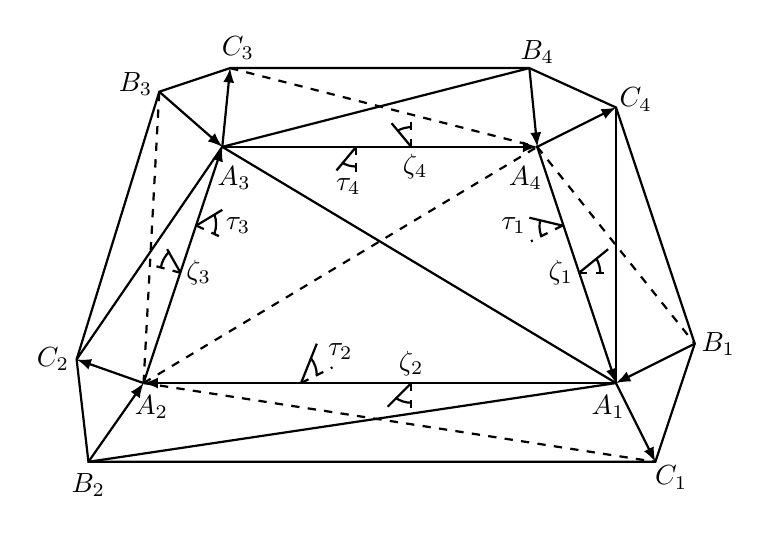
\begin{tikzpicture}[>=latex]              %\draw[help lines] (0,0) grid (15,10);

        \coordinate (a1) at (9, 4);
        \coordinate (a2) at (3, 4);
        \coordinate (a3) at (4, 7);
        \coordinate (a4) at (8, 7);
        \coordinate (b1) at (10, 4.5);
        \coordinate (c1) at (9.5, 3);
        \coordinate (b2) at (2.3, 3);
        \coordinate (c2) at (2.15, 4.3);
        \coordinate (b3) at (3.2, 7.7);
        \coordinate (c3) at (4.1, 8);
        \coordinate (b4) at (7.9, 8);
        \coordinate (c4) at (9, 7.5);

        \draw[thick] (a1) edge[->] (a2) (a2) edge[->] (a3) (a3) edge[->] (a4) (a4) edge[->] (a1);
        
        \draw[dashed, thick] (a2) -- (a4);
        \draw[thick] (a3) -- (a1);
        
        
        \draw[thick] (b1) -- (c1) -- (b2) -- (c2) -- (b3) -- (c3) -- (b4) -- (c4) -- cycle;
        
        \draw[thick, <-] (a1) -- (b1);
        \draw[thick, ->] (a1) -- (c1);
        
        \draw[thick, <-] (a2) -- (b2);
        \draw[thick, ->] (a2) -- (c2);
        
        \draw[thick, <-] (a3) -- (b3);
        \draw[thick, ->] (a3) -- (c3);

        \draw[thick, <-] (a4) -- (b4);
        \draw[thick, ->] (a4) -- (c4);

        \draw[thick] (a1) -- (c4); 
        \draw[thick, dashed] (a4) -- (b1);
        
        \draw[thick, dashed] (a2) -- (c1);
        \draw[thick] (a1) -- (b2);

        \draw[thick, dashed] (a2) -- (b3);
        \draw[thick] (c2) -- (a3);

        \draw[thick, dashed] (c3) -- (a4);
        \draw[thick] (b4) -- (a3);

        \draw (a1) + (-0.1, -0.3) node {$A_1$};
        \draw (b1) + (0.3, 0) node {$B_1$};
        \draw (c1) + (0.2, -0.2) node {$C_1$};
        
        \draw (a2) + (0.1, -0.3) node {$A_2$};
        \draw (b2) + (0, -0.3) node {$B_2$};
        \draw (c2) + (-0.3, 0) node {$C_2$};
        
        \draw (a3) + (0.15, -0.4) node {$A_3$};
        \draw (b3) + (-.3, 0.1) node {$B_3$};
        \draw (c3) + (0.1, .25) node {$C_3$};
        
        \draw (a4) + (-0.15, -0.4) node {$A_4$};
        \draw (b4) + (0.1, 0.2) node {$B_4$};
        \draw (c4) + (.25, .1) node {$C_4$};

        \draw[thick, dashed] (5, 4) -- (5.4, 4.2);
        \draw[thick] (5, 4) -- (5.2, 4.5);
        \draw[thick] (5.2,4.1) arc (0:39:10pt);
        \draw (5.5, 4.4) node {$\tau_2$};

        \draw[thick] (6.4, 4) -- (6.1, 3.7);
        \draw[thick, dashed] (6.4, 4) -- (6.4, 3.65);
        \draw[thick] (6.4, 3.75) arc (270:235:10pt);
        \draw (6.4, 4.25) node {$\zeta_2$};

        \draw[thick] (8.53, 5.4) -- (8.9, 5.7);
        \draw[thick, dashed] (8.53, 5.4) -- (8.9, 5.4);
        \draw[thick] (8.8, 5.4) arc(0:30:10pt);
        \draw (8.3, 5.4) node {$\zeta_1$};

        \draw[thick, dashed] (8.32, 6) -- (7.92, 5.8);
        \draw[thick] (8.32, 6) -- (7.9, 6.1);
        \draw[thick] (8.05, 5.87) arc(200:167:10pt);
        \draw[thick] (7.7, 6) node {$\tau_1$};
        
        \draw[thick] (6.4, 7) -- (6.15, 7.3);
        \draw[thick, dashed] (6.4, 7) -- (6.4, 7.4);
        \draw[thick] (6.4, 7.25) arc (90:120:10pt);
        \draw (6.45, 6.75) node {$\zeta_4$}; 

        \draw[thick, dashed] (5.7, 7) -- (5.7, 6.6);
        \draw[thick] (5.7, 7) -- (5.45,6.7);
        \draw[thick] (5.7, 6.75) arc(270:240: 10pt);
        \draw (5.6, 6.5) node {$\tau_4$};

        %\draw[thick] (3.7, 6) node {\textbullet};
        \draw[thick, dashed] (3.47, 5.4) -- (3.1, 5.5);
        \draw[thick] (3.47, 5.4) -- (3.3, 5.7);
        \draw[thick] (3.22, 5.47) arc(170:132:10pt);
        \draw (3.7, 5.4) node {$\zeta_3$};

        \draw[thick] (3.67, 6) -- (4, 6.2);
        \draw[thick, dashed, rotate around ={-25:(3.67, 6)} ] (3.67, 6) -- (4, 6);
        \draw[thick] (3.9, 5.9) arc (-20:20:10pt);
        \draw (4.2, 6) node {$\tau_3$};
    \end{tikzpicture}